\section{Experiments}
\label{sec:experimental}

\subsection{Experiment 1: forced-choice}
\label{sec:exp:fc}

In the two experiments reported in this section, I use probabilities for the alternating constructions calculated for attested material, and I correlate these probabilities with the participants' reactions.
Thus, a direct link can be established between output material found in corpora and the behaviour of linguistic agents.
Both experiments use sentences containing attested MNPs from the corpus sample (embedded into simplified sentences) as stimuli.

Readers might wonder why the stimuli were chosen in such a way.
Alternatively, one could have created stimuli where the features favouring the alternatives were permuted appropriately and thus tested directly.
The answer is related to what was said in Section~\ref{sec:cogocl} about the rich multi-factorial data sets used in corpus studies and the comparatively restricted ones in experiments.
Looking at Table~\ref{tab:variables}, we see one binary factor (\textit{Cardinal}), two three-level factors (\textit{Measurecase} and \textit{Kindgender}) and one five-level factor (\textit{Measureclass}).
Since the dependent variable is binary (\textit{Construction}), permuting these factors alone leads to 180 different possible permutations.
On top of this, the numeric variables \textit{Kindattraction} and \textit{Measureattraction} would also have to be tested at at least two or three different values each.
It is obvious that this is impossible in a controlled experiment, given that participants can usually be exposed to something in the region of one hundred sentences (including many more fillers than target stimuli) within thirty minutes to an hour.
Thus, while the present approach only allows for a global test of the corpus-derived model, this appears to me to be the only feasible way.%
\footnote{Obviously, the experimental data are much too sparse to perform even post-hoc analyses with respect to the single regressors in a statistically and scientifically sound way.}
It is, in the sense of Section~\ref{sec:cogocl}, an optimal synthesis of data-rich multifactorial corpus studies and experimental validation, and it is one that has been used (although rarely; see \citealp[3--4]{DivjakEa2016a}) at least since the seminal \citet{BresnanEa2007} paper.

\subsubsection{Setup, stimuli, and participants}

The first experiment tests preferences for constructions explicitly in a forced choice task.
% \cite{FordBresnan2013} use the \textit{split-100} task in which participants have to distribute 100 points between the alternatives, assigning more points to more natural sounding alternative.
% In essence, participants distribute a probability mass between two alternants, which is intended to produce more subtle results compared to a two-alternative forced-choice task such as in \cite{Rosenbach2013}, where participants have to choose one of two alternants.
% The split-100 paradigm has been criticised in \cite{ArppeJaervikivi2007}.
% The criticism was reiterated in \cite{DivjakEa2016}, where they use a forced-choice task.
% In \cite{VerhoevenTemme2017}, it was shown that results from forced-choice and split-100 experiments mostly converge (with some numeric intricacies related to the non-linear distribution of preferences for alternants).
% I present a forced-choice experiment in this section instead of a split-100 experiment not only because of some researchers' critical attitude towards the split-100 task, but also because in a dry run of the experiment, participants complained about the unnaturalness of distributing a probability mass across two alternants and tended to produce ratings of 0 or 100 (or 50, although to a lesser degree).
Participants had to choose between two sentences that differed only in that one contained the \NACa\, and the other one contained the \PGCa.
The analysis compares the probabilities assigned to the stimuli by the corpus-derived model with the frequency with which participants chose the alternants.
There were 24 participants (native speakers of German without reading or writing disabilities) aged 19 to 30 living permanently in [NAME OF CITY REDACTED], who were recruited from introductory linguistics courses at [NAME OF UNIVERSITY REDACTED].
Although the experiment was conducted in the last four weeks of their first semester, participants had no deeper explicit knowledge of linguistics, grammar, or experimental methods.
None of them had ever participated in a forced-choice experiment before.
Participation was voluntary but participants received credit in partial fulfillment of course requirements.

As stimuli, attested MNPs from the corpus study were used, but the sentences were radically simplified to avoid influences from contextual nuisance factors as much as possible.
The approach is also justified because according to the theoretical assessment in Section~\ref{sec:analyses}, the choice of alternants depends mostly on a very local constructional context.
I sampled 16 MNPs from the concordance and made sure that the simplifications and normalisations did not affect any of the regressors used in the corpus study.
In the simplified sentences, the case, number, etc. of the MNP remained the same as in the attested sentence, as did the choice of lexical material within the MNP.
Eight sentences contained masculine or neuter kind nouns, and the other eight contained feminine kind nouns.
Furthermore, in each of the masculine\slash neuter and feminine groups, four sentences originally containing the \NACa\ and four sentences originally containing the \PGCa\ were chosen.
More precisely, the sentences were sampled as \textit{highly typical examples} of \PGCa\ (high probability assigned by GLMM) and \NACa\ (low probability assigned by GLMM), respectively.%
\footnote{Remember from Section~\ref{sec:corpusstudies} that the model predicts the probability that the \PGCa\ is chosen over the \NACa.}
High and low probabilities were defined as the top and bottom 20\% of all probabilities assigned by the GLMM.
Lemmas and feature combinations were made unique within each group whenever possible.
The design is summarised in Table \ref{tab:experiment1:design}.

\begin{table}
  \centering
  \begin{tabular}[h]{lll}
     & Masculine\slash Neuter & Feminine \\
     \midrule
     \textbf{high prob.\ for PGC\Subsf{adj}} & 4 sentences & 4 sentences \\
     \textbf{low prob.\ for PGC\Subsf{adj}} & 4 sentences & 4 sentences \\
  \end{tabular}
  \caption{The four groups of sentences chosen as stimuli; in each group of four sentences, combinations of important factor values were made unique whenever possible}
  \label{tab:experiment1:design}
\end{table}

The final pairs of stimuli were the sentence containing the attested and preferred alternant (according to the corpus GLMM) on the one hand and a modified version containing the dispreferred alternant on the other hand.
They were presented next to each other, and a 20 second time limit for each choice was set.%
\footnote{No participant ever exceeded the time limit.}
The position on the screen (left\slash right) and the order of sentences were randomised for each participant.
As fillers, 23 pairs of sentences exemplifying similar but unrelated alternation phenomena from German morpho-syntax were used.
Thus, participants saw 39 pairs of sentences and 78 sentences in total.
They were instructed to select from each pair of sentences the one that seemed more natural to them in the sense that they would use it rather than the other one.
The experiment was conducted using \textit{PsychoPy} \citep{Peirce2007}.

\subsubsection{Statistical model}

\begin{figure}[htbp!]
\centering
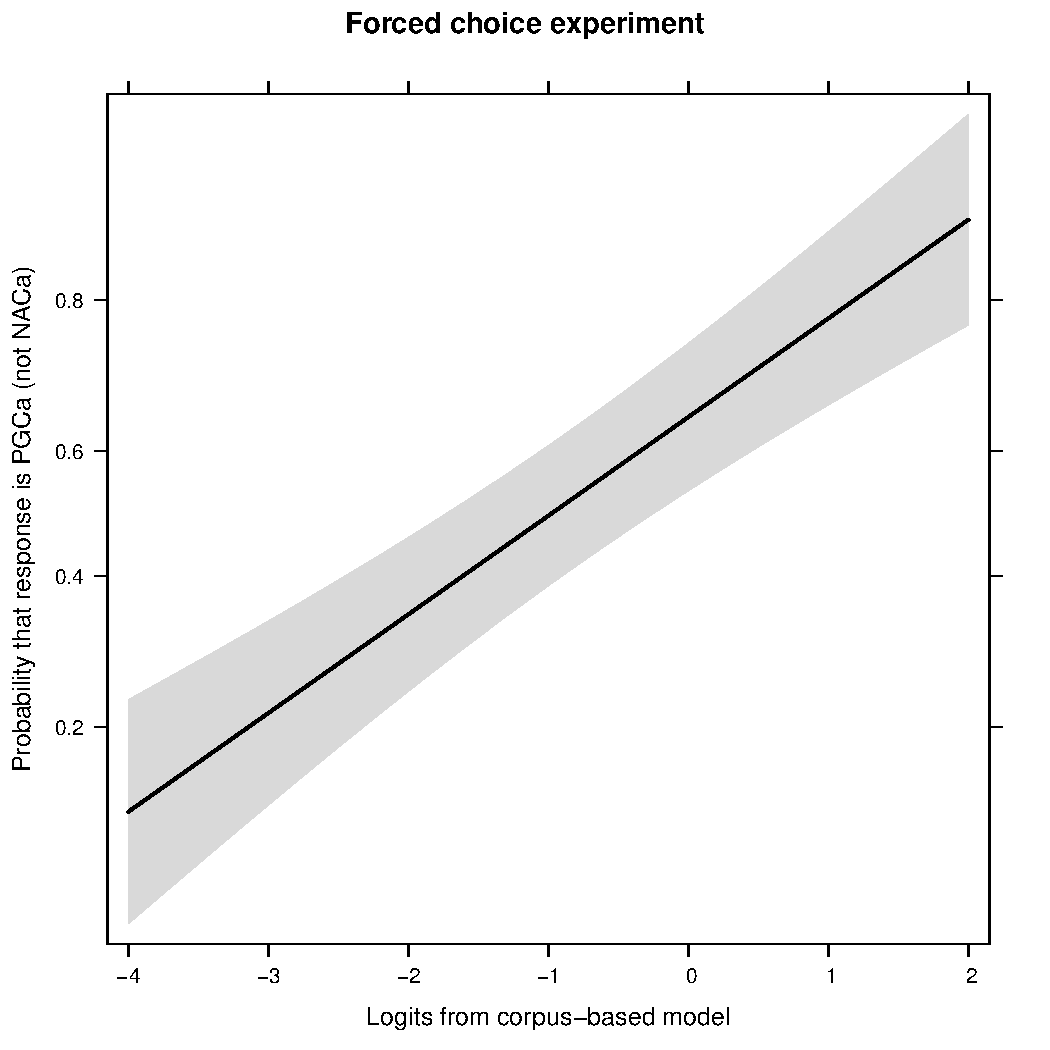
\includegraphics[width=0.5\textwidth]{../R/output/fc_effects}
\caption{Effect plot for the multilevel logistic regression in the forced-choice experiment: predictability of participants' choices using the probabilities derived from the corpus-based GLMM}
\label{fig:afc:effects}
\end{figure}

A multilevel logistic regression was specified with the probability of the \PGCa\ predicted for each sentence by the corpus-based GLMM as the only fixed effect \textit{Modelprediction}.%
\footnote{The document-level variables \textit{Badness} and \textit{Genitives} were set to 0, which is the mean for z-transformed variables.}
A random intercept and slope were added for the individual sentence pair (item) in order to catch idiosyncrasies of single sentences.
Coefficients were estimated with Maximum Likelihood Estimation (\textit{lmer} function from \textit{lme4}).
The number of observations was \textit{n=}384.

A good amount of the variance can be accounted for by idiosyncrasies of single sentences ($\sigma_{\text{Item}}=1.217$).
Also, among participants, there are clearly different preferences ($\sigma_{\text{Participant}}=0.412$).
On the extreme ends, one participant chose the \PGCa\ in 13 of 16 cases, and two participants only chose it in 5 of 16 cases.
The regressor \textit{Modelprediction} achieves $\mpPB=0.003$ (1,000 replications) and is estimated at 4.389 relative to an intercept of -1.270.
The confidence interval from a parametric bootstrap (1,000 replications, percentile method) for the regressor is acceptable but a tad large with a lower bound of 1.788 and an upper bound of 6.599.
The pseudo-coefficients of determination are $R^2_{m}=0.185$ and $R^2_{c}=0.455$, which means that roughly 19\% of the variance in the data can be explained by considering only the predictions from the corpus-based GLMM.

\subsubsection{Interpretation}

The coefficients of determination indicate a weak result for the fixed effects part of the model, which is nonetheless worthy of mention (very close to 0.2).
The effect display for the single fixed regressor \textit{Modelprediction} is given in Figure \ref{fig:afc:effects}.
The higher the probability of the \PGCa\ predicted from usage data, the more often participants chose the \PGCa\ alternant in the forced-choice task.
A closer look at the results in the form of the spineplot in Figure~\ref{fig:spines} shows, however, that it was likely an idiosyncracy of a single sentence with a probability predicted by the model between 0.5 and 0.6 which spoiled an otherwise much better correlation.
The problematic sentence with a model prediction of 0.548 is given in (\ref{ex:problem}) in the \PGCa\ variant.

\begin{exe}
  \ex{\label{ex:problem}\gll Man machte mal wieder viel Lärm um [jede Menge [heißer Luft]\Sub{Gen}]\Sub{Acc}.\\
  one made once again much noise about any amount hot air\\
  \trans People made much ado about nothing once again.}
\end{exe}

In retrospect, this stimulus was badly chosen because \textit{heiße Luft} `ado' (literally `hot air') is a fixed metaphorical expression.
This obviously influences the reactions of participants, and a revised and improved experiment might lead to a much better fit in future research.

\begin{figure}[htbp!]
  \centering
  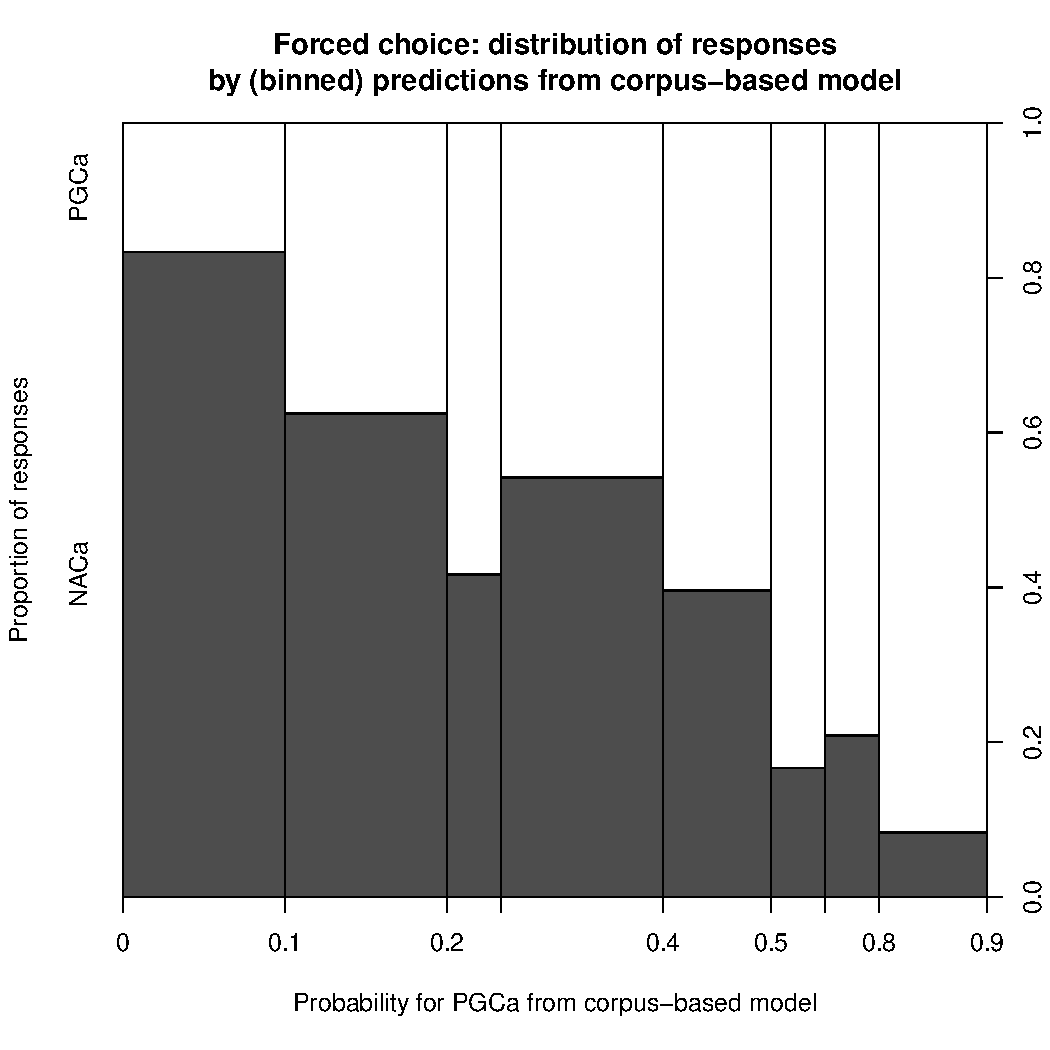
\includegraphics[width=0.5\textwidth]{../R/output/fc_proportions}
  \caption{Spineplot of the proportion of responses plotted against the predictions from the corpus-based model in the forced-choice experiment}
  \label{fig:spines}
\end{figure}

In principle, random slope for \textit{Modelprediction} varying by item could also remedy problems with individual stimuli at least partially.
Therefore, a model with random slopes for \textit{Modelprediction} varying by both random effects (\textit{Participant} and \textit{Item}) was specified and estimated.
The random slope for participants was added to comply with \citet[257]{BarrEa2013} who predict ``catastrophically high Type I error rates'' for experimental designs with within-subject manipulations if random effects structures are not kept maximal.
The coefficient of the fixed effect changed noticeably but not enough to change the interpretation (5.408 relative to an intercept of -1.304), and the marginal $R^2_m$ rises to 0.213 ($R^2_c=0.488$).
In line with expectations, the standard deviation in the random slopes for \textit{Item} is high at 5.996.
However, the covariance parameters were estimated at -1.0, which is a clear sign that the variance-covariance matrix could not be estimated successfully.
The same was true for models with only an \textit{Item} and a \textit{Participant} random slope.
This is exactly the kind of model overparametrisation criticised in \citet{BatesEa2015a} and \citet{MatuschekEa2017}.
The available data are insufficient to estimate the parameters of the more complex model with varying slopes.%
\footnote{\citet[1]{BatesEa2015a} state: ``We show that failure to converge typically is not due to a suboptimal estimation algorithm, but is a consequence of attempting to fit a model that is too complex to be properly supported by the data, irrespective of whether estimation is based on maximum likelihood or on Bayesian hierarchical modeling with uninformative or weakly informative priors.
Importantly, even under convergence, overparameterization may lead to uninterpretable models.''
}

In summary, the forced-choice experiment succeeded in corroborating the results from the corpus study inasmuch as the preferences extracted from usage data correspond to native speakers' choices, but the correlation is weak, likely at least in part due to problems with individual test items and\slash or too sparse data.


\subsection{Experiment 2: self-paced reading}
\label{sec:exp:spr}

\subsubsection{Setup, stimuli, and participants}

The second experiment tests preferences more implicitly.
It is expected that reading less typical alternants in a given context and with given lexical material incurs a processing overhead for the reader (\citealp{Kaiser2013}).
In this section, a self-paced reading experiment is therefore presented.
In a very similar fashion, \cite{DivjakEa2016} apply the self-paced reading paradigm in the validation of corpus-based models.
The analysis compares the corpus-derived probabilities with potential lags in reading time for sentences with the preferred and the non-preferred constructions.

Concretely, the exact same stimuli as in the forced-choice experiments were used.
Each participant read both the 16 sentences with the alternant predicted by the corpus model and the 16 modified sentences with the alternant that the corpus model did not predict.%
\footnote{Notice that lemmas and their frequencies as well as lemma classes are included as regressors in the corpus-based GLMM, and there was consequently no additional controlling of lemma frequencies, etc.}
To minimise repetition effects, the stimuli for each participant were separated into two blocks of 16 targets and 33 fillers per block.
In the experiment, participants first read all sentences from the first block, then all sentences from the second block.
From each target sentence pair, one sentence was assigned to the first block and the other sentence to the other block.
The assignment of members of the individual sentence pairs to the blocks was randomised for each participant individually, as was the order within each block.
The fillers also came in pairs such that the second block exclusively contained sentences to which participants had been exposed in the first block in slightly modified form.
In total, each participant read 98 sentences.
After each sentence, participants had to answer simple (non-metalinguistic) yes-no questions about the previous sentence as distractors.
The distractor questions were different between the first and the second blocks.
There were 38 participants recruited in exactly the same manner as for the experiment reported in Section~\ref{sec:exp:fc}.
None of them had ever participated in any kind of reading experiment, and none of them took part in the first experiment.
The experiment was conducted using \textit{PsychoPy}.

The reading times were residualised per speaker based on the reading times of all words (not just the targets) by that speaker.
The adjective and the kind noun (\ie\ the constituents bearing the critical case markers) were used as the target region, for instance the bracketed words in the example \textit{zwei Gläser} [\textit{spru\-deln\-des Wasser}] `two glasses of sparkling water'.
Outliers farther than 2 inter-quartile ranges from the mean logarithmised residualised reading time were removed (64 data points), resulting in a total number of \textit{n=}1,152 observations.

\subsubsection{Statistical model}

An LMM was specified with the logarithmised residual reading times as the response variable.
The probabilities derived from the corpus GLMM (\textit{Modelprediction}) were added as the main regressor of interest.
It should be remembered that the corpus GLMM predicts the probability of the \PGCa.
As a consequence, the higher the GLMM prediction is, the more typical the sentence is for containing the \PGCa.
It is therefore expected that reading times are higher when the value of \textit{Modelprediction} is higher but the sentence contains the \NACa.
However, when the sentence contains the \PGCa, reading times should be lower when \textit{Modelprediction} is higher.
To account for this, an interaction between \textit{Modelprediction} and \textit{Construction} (levels \textit{PGCadj} and \textit{NACadj}) was added to the model.

Furthermore, the position (1--98) of the sentence in the individual experiment (\textit{Position}) was included as a fixed effect to control for the usual increase in reading speed during an experiment run.
Random intercepts were specified for \textit{Participant} and \textit{Item} (the 16 sentence pairs are one \textit{Item} each).%
\footnote{Again, all attempts to include random slopes resulted in the variance-covariance matrix not being properly estimated (1 or -1 covariance parameters).}

\begin{table}
  \centering
  \begin{tabular}{lrrrc}
    Regressor & \multicolumn{1}{r}{Coefficient} & \multicolumn{1}{r}{CI low} & \multicolumn{1}{r}{CI high} & \multicolumn{1}{r}{CI excludes 0} \\ \midrule
    Construction=PGCadj                 &  0.054 &  0.012 &  0.095 &  *  \\ 
    Modelprediction                     & -0.003 & -0.113 &  0.110 &     \\ 
    Position                            & -0.005 & -0.005 &  0.004 &     \\ 
    Construction=PGCadj:Modelprediction & -0.125 & -0.234 & -0.023 &  *  \\ 
  \end{tabular}
  \caption{Fixed effect coefficient table for the LMM used to analyse the self-paced reading experiment; the intercept is 0.829}
  \label{tab:exp:spr}
\end{table}

Table~\ref{tab:exp:spr} shows the coefficient estimates with a 95\% parametric bootstrap confidence interval (1,000 replications, percentile method).
The standard deviation of the participant intercepts is $\sigma_{\text{Participant}}=0.079$ and of the item intercepts $\sigma_{\text{Item}}=0.037$.
Comparing the full model to a model without the main regressor \textit{Modelprediction} (and consequently also without the interaction with \textit{Construction}) in a PBmodcomp test gives $\mpPB=0.036$.
The pseudo-coefficients of determination are $R^2_m=0.239$ and $R^2_c=0.346$.

An alternative Gaussian generalised additive model with an identity link was also fit (see \citealp{DivjakEa2016}) using the \textit{mgcv} package \citep{Wood2011}.
The full results are included in the data package for this paper, but the fit was not better than with the LMM reported above.
The estimated smoother for the \textit{Modelprediction} variable is essentially linear, and the $R^2$ (corresponding to the marginal $R^2$ of the LMM) was 0.237.

\subsubsection{Interpretation}

The coefficients of determination indicate that there is a noteworthy correlation between the reactions of the subjects and the corpus-derived probabilities (marginal $R^2$) and that there is some between-subject variation (conditional minus marginal $R^2$).

\begin{figure}[htbp!]
\centering
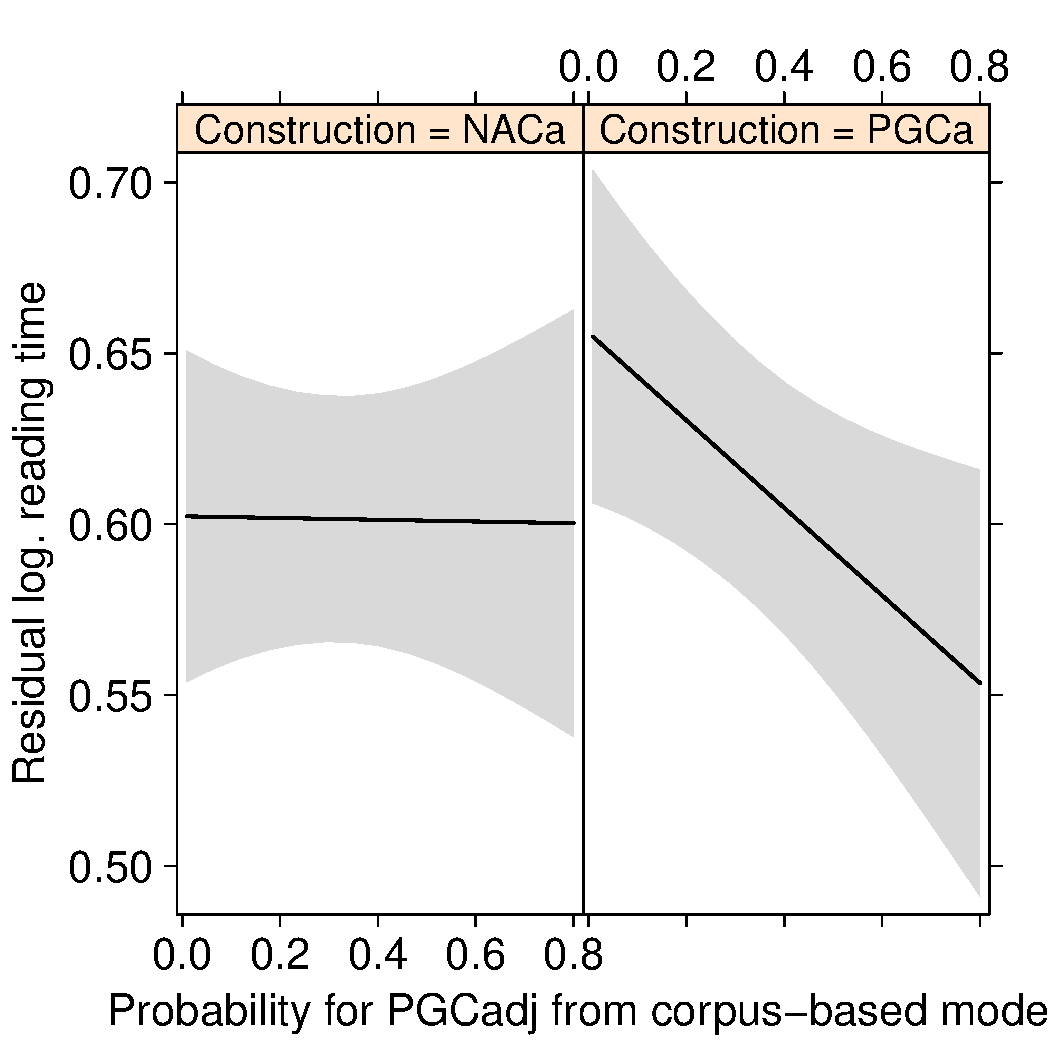
\includegraphics[width=0.5\textwidth]{../R/output/spr_effects}
\caption{Effect plot for the LMM in the self-paced reading experiment: modeling participants' residualised log reading times on the probabilities given by the corpus-based GLMM}
\label{fig:spr:effects}
\end{figure}

The effect plot for the interaction of interest is shown in Figure~\ref{fig:spr:effects}.
The estimate for the sentences with \NACa\ is obviously imprecise, and no significant differences in reading times are observed.
There is a clearer effect in the sentences with \PGCa, which is also confirmed by the significant results from the bootstrapped confidence intervals (see Table~\ref{tab:exp:spr}) and from the PBmodcomp test reported above.
The \PGCa\ brings about an increased reading time, which is plausible because it is the much rarer construction (see Section~\ref{sec:corpusstudies}).
However, if it occurs in a prototypical context and with typical lexical material, reading times drop.
This can be seen in the downward slope in the right panel of Figure~\ref{fig:spr:effects}.
This fits into the general picture inasmuch as the construction with the lower frequency might be developing towards a more sharply defined prototype.%
\footnote{In this context, it should be remembered from Section~\ref{sec:corpusstudies} that even the \PGCd\ is much rarer that the \NACb\ (17,252 vs.\ 315,635 occurrences in the auxiliary corpus samples).}
Conversely, the \NACa\ (like the NAC in general) might be the highly frequent default which does not incur a reading time penalty, even if it is not the optimal choice in the given context and with the given lexical material.

In Section~\ref{sec:conclusion}, I take stock and summarise the contributions of the present study to the research on alternations in cognitive linguistics.
